\documentclass{beamer}
\newlength\mywd
\setlength\mywd{1cm}
\usetheme[]{Warsaw}
\usefonttheme[onlymath]{serif}
\usepackage[polish]{babel}
\usepackage[utf8]{inputenc}
\usepackage{polski}
\usepackage[T1]{fontenc}
\usepackage{times} % Używa czcionek wektorowych
\usepackage{indentfirst}
\usepackage{psfrag}
\usepackage{graphicx}
\usepackage{epstopdf}
\usepackage{enumitem}
\usepackage{hyperref}
\graphicspath{ {./images/} }
\frenchspacing
% Titlepage
\title{Mean Shift}
\author{Marcin Lembke}
\date{24 listopada 2014}
%
% Beamer settings
\definecolor{primary}{RGB}{32,46,109}
\definecolor{secondary}{RGB}{20,130,180}
\setbeamercolor*{palette primary}{use=structure,fg=white,bg=primary}
\setbeamercolor*{palette secondary}{use=structure,fg=white,bg=primary}
\setbeamercolor*{palette quaternary}{fg=black,bg=secondary}
\setbeamercolor{frametitle}{bg=primary}     %controls the color of the headline
\setbeamercolor{sidebar}{bg=primary}        %controls the color of the sidebar
\setbeamercolor{logo}{bg=primary}  %controls the color of the logo area
%
\addtobeamertemplate{navigation symbols}{}{%
	\usebeamerfont{footline}%
	\usebeamercolor[fg]{footline}%
	\hspace{1em}%
	\insertframenumber/\inserttotalframenumber
}
\setbeamercolor{footline}{fg=blue}
\setbeamerfont{footline}{series=\bfseries}
\newcommand{\norm}[1]{\left\lVert#1\right\rVert}
\setitemize{label=\usebeamerfont*{itemize item}
	\usebeamercolor[fg]{itemize item}
	\usebeamertemplate{itemize item}}
\setenumerate[1]{%
	label=\protect\usebeamerfont{enumerate item}%
	\protect\usebeamercolor[fg]{enumerate item}%
	\insertenumlabel.}

\usepackage[absolute,overlay]{textpos}

\setbeamercolor{framesource}{fg=gray}
\setbeamerfont{framesource}{size=\tiny}

\newcommand{\source}[1]{\begin{textblock*}{4cm}(8.7cm,8.6cm)
		\begin{beamercolorbox}[ht=0.5cm,right]{framesource}
			\usebeamerfont{framesource}\usebeamercolor[fg]{framesource} Źródło: {#1}
		\end{beamercolorbox}
	\end{textblock*}}
	
\newcommand{\adapted}[1]{\begin{textblock*}{4cm}(8.7cm,8.6cm)
		\begin{beamercolorbox}[ht=0.5cm,right]{framesource}
			\usebeamerfont{framesource}\usebeamercolor[fg]{framesource} Zaadaptowano z: {#1}
		\end{beamercolorbox}
	\end{textblock*}}
%gets rid of navigation symbols
\setbeamertemplate{navigation symbols}{}
\setbeamertemplate{headline}{}
\begin{document}
	\maketitle
	\begin{frame}
		\frametitle{Agenda}
		\tableofcontents
	\end{frame}
	
	\section{Czym jest Mean Shift?}
	\begin{frame}
		\begin{beamercolorbox}[colsep=-4bp,rounded=true,shadow=true,ht=0.5cm,dp=0.3cm,center]{title}
			\usebeamerfont{title} \usebeamercolor*[fg]{title} Czym jest Mean Shift?
		\end{beamercolorbox}
	\end{frame}
	
	\begin{frame}
		\frametitle{Czym jest Mean Shift?}
		\begin{itemize}
			\item Po raz pierwszy zaprezentowany przez K. Fukunagę oraz L. Hostetlera\footnote{Fukunaga, Keinosuke; Larry D. Hostetler (January 1975). "The Estimation of the Gradient of a Density Function, with Applications in Pattern Recognition".}, 
			\item Algorytm iteracyjny,
			\item Pozwala na znalezienie lokalnych maksimów rozkładu gęstości wybranej cechy,
			\item Efektywny w zastosowaniach śledzenia obiektów, których cechy można przestawić za pomocą histogramów.
		\end{itemize}
	\end{frame}
	
	\subsection{Podejście intuicyjne}
	\begin{frame}
		\begin{beamercolorbox}[colsep=-4bp,rounded=true,shadow=true,ht=1cm,dp=0.3cm,center]{title}
			\usebeamerfont{title} \usebeamercolor*[fg]{title} Czym jest Mean Shift?\\
			\usebeamerfont{subtitle} \usebeamercolor*[fg]{subtitle} Podejście intuicyjne
		\end{beamercolorbox}
	\end{frame}
	
	\begin{frame}
		\frametitle{Czym jest Mean Shift?}
		\framesubtitle{Podejście intuicyjne}
		\begin{figure}[H]
			\centering
			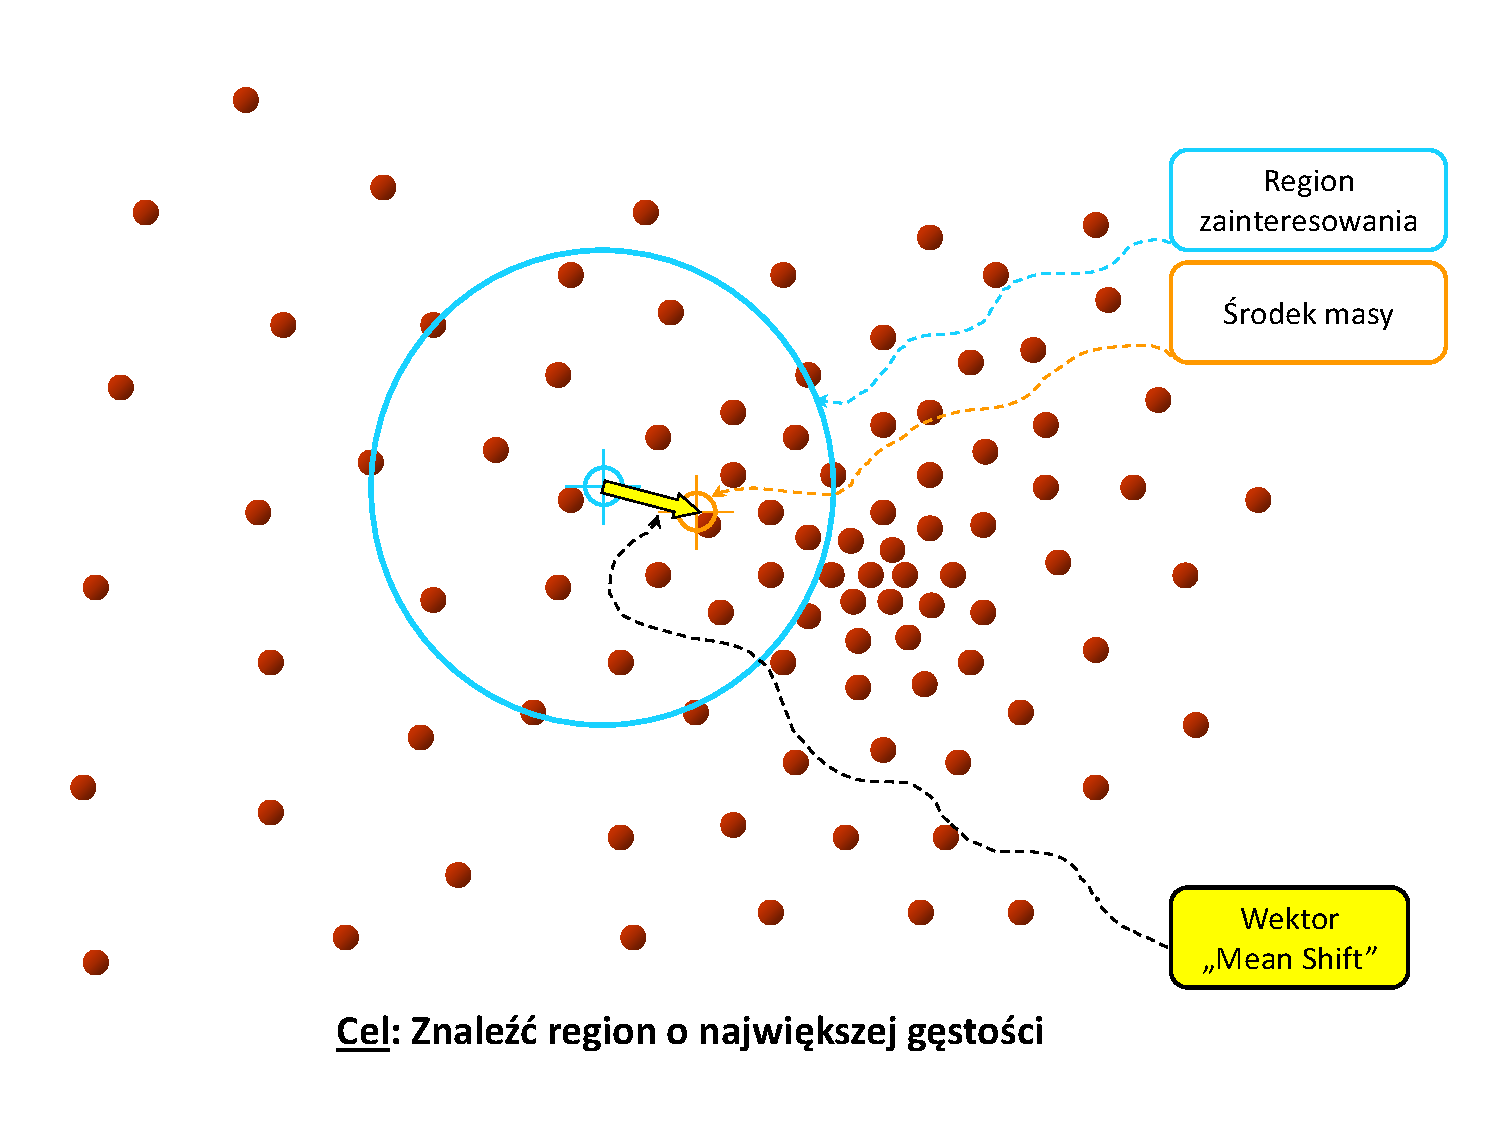
\includegraphics[width=0.9\textwidth]{mean_shift_intuitive_1.pdf}
			\adapted{\href{http://www.wisdom.weizmann.ac.il/~vision/courses/2004_2/files/mean_shift/mean_shift.ppt}{Ukrainitz, Y., Sarel, B.}}
		\end{figure}
	\end{frame}
	
	\begin{frame}
		\frametitle{Czym jest Mean Shift?}
		\framesubtitle{Podejście intuicyjne}
		\begin{figure}[H]
			\centering
			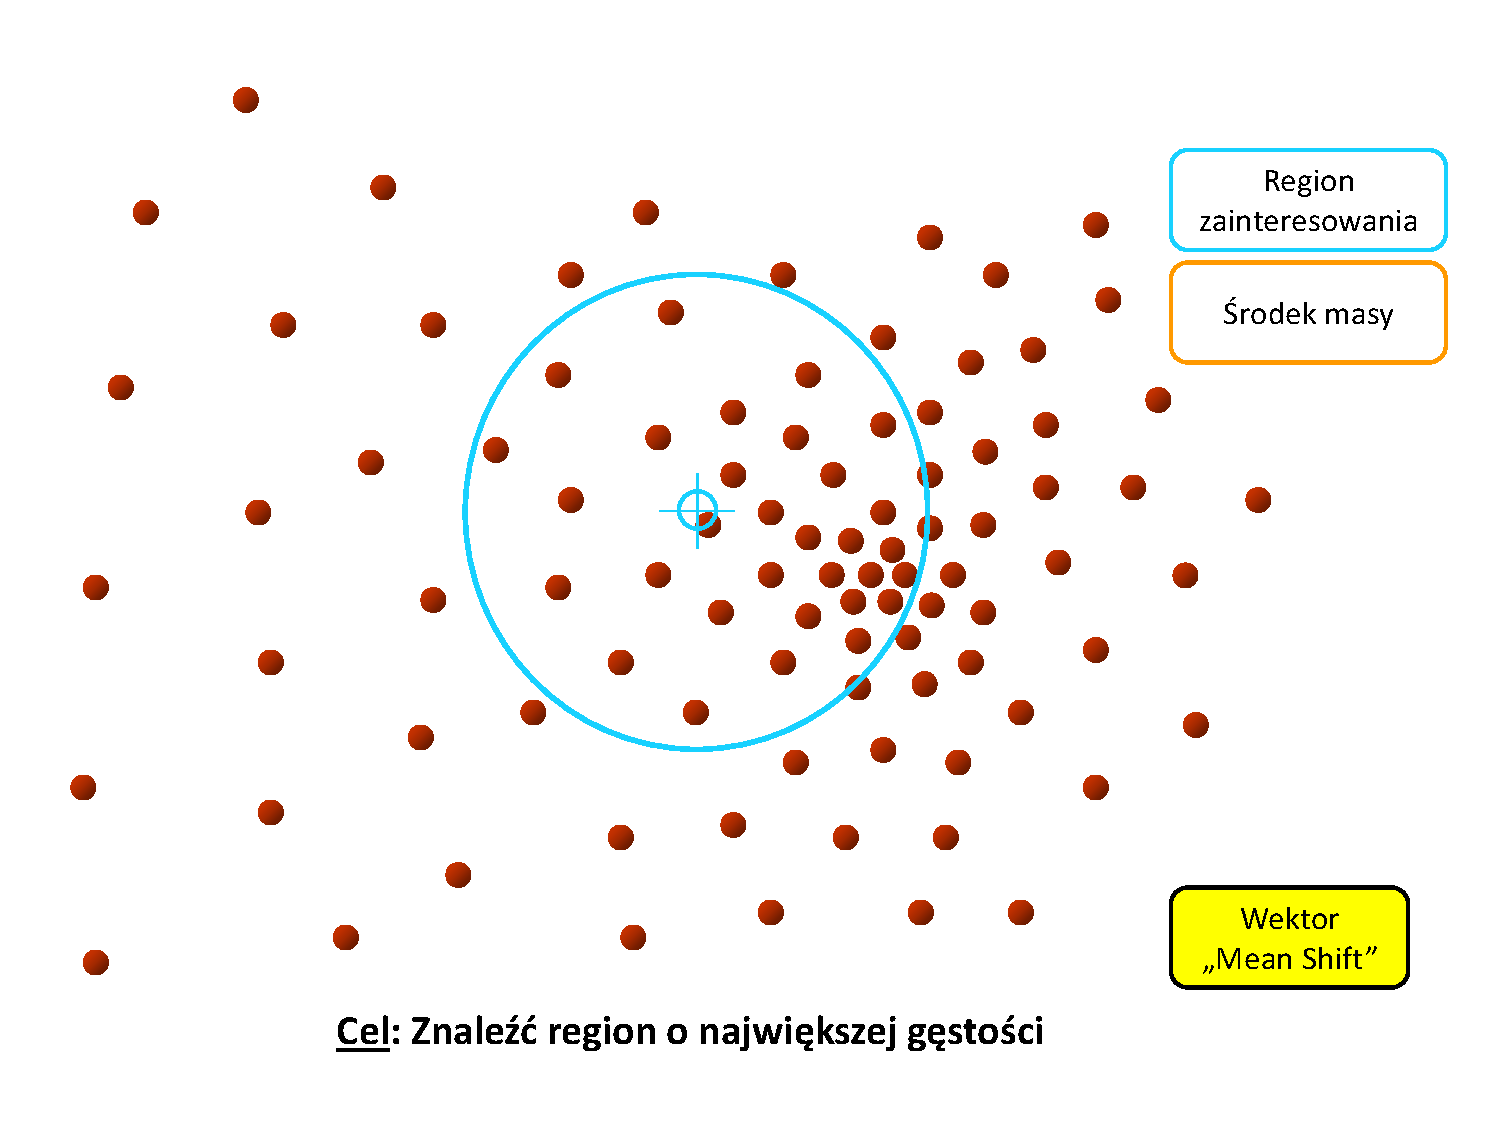
\includegraphics[width=0.9\textwidth]{mean_shift_intuitive_2.pdf}
			\adapted{\href{http://www.wisdom.weizmann.ac.il/~vision/courses/2004_2/files/mean_shift/mean_shift.ppt}{Ukrainitz, Y., Sarel, B.}}
		\end{figure}
	\end{frame}
	
	\begin{frame}
		\frametitle{Czym jest Mean Shift?}
		\framesubtitle{Podejście intuicyjne}
		\begin{figure}[H]
			\centering
			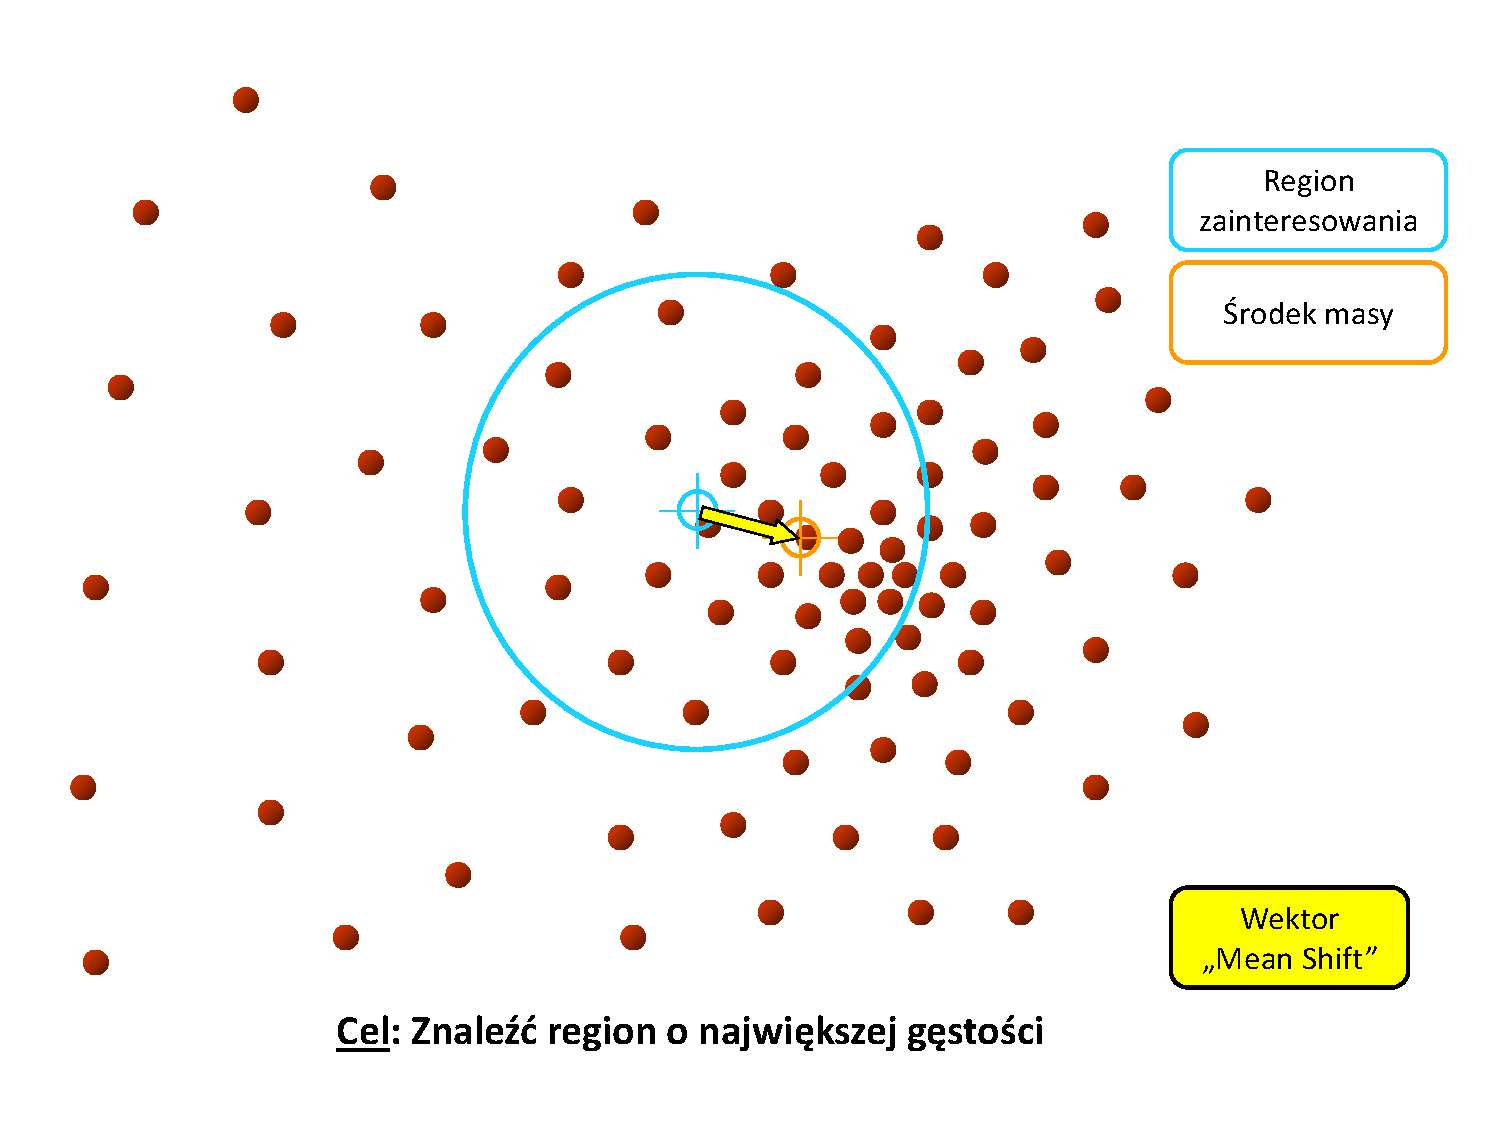
\includegraphics[width=0.9\textwidth]{mean_shift_intuitive_3.pdf}
			\adapted{\href{http://www.wisdom.weizmann.ac.il/~vision/courses/2004_2/files/mean_shift/mean_shift.ppt}{Ukrainitz, Y., Sarel, B.}}
		\end{figure}
	\end{frame}
	
	\begin{frame}
		\frametitle{Czym jest Mean Shift?}
		\framesubtitle{Podejście intuicyjne}
		\begin{figure}[H]
			\centering
			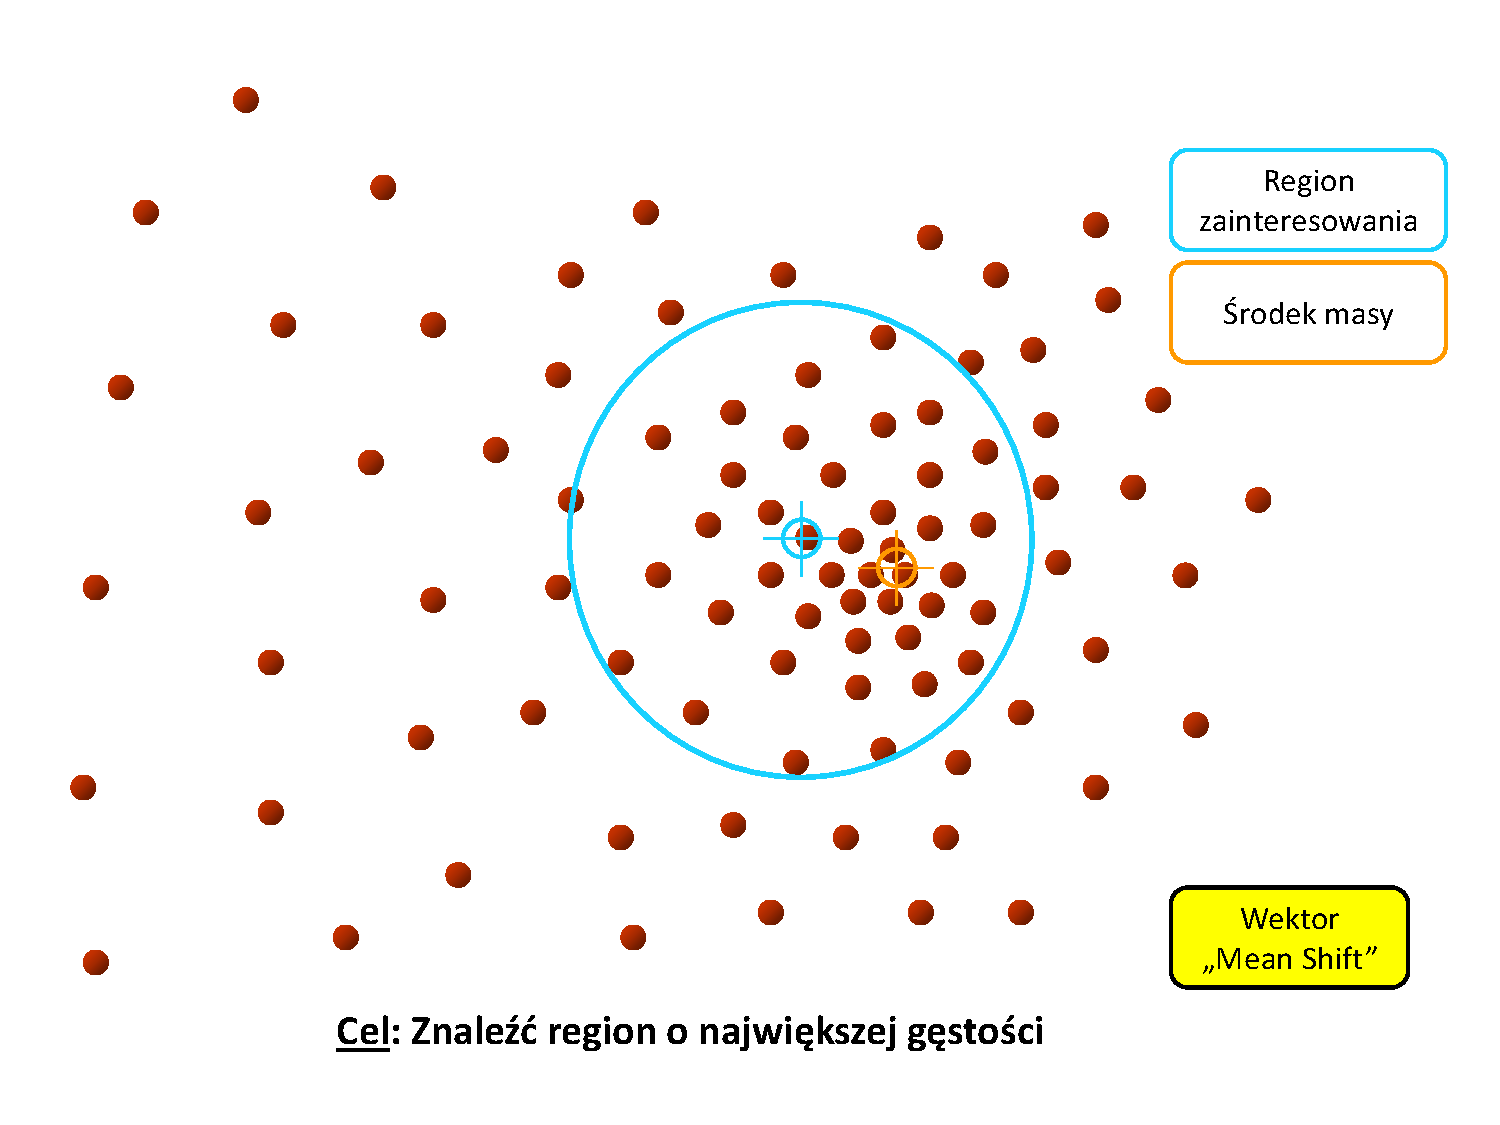
\includegraphics[width=0.9\textwidth]{mean_shift_intuitive_4.pdf}
			\adapted{\href{http://www.wisdom.weizmann.ac.il/~vision/courses/2004_2/files/mean_shift/mean_shift.ppt}{Ukrainitz, Y., Sarel, B.}}
		\end{figure}
	\end{frame}
	
	\begin{frame}
		\frametitle{Czym jest Mean Shift?}
		\framesubtitle{Podejście intuicyjne}
		\begin{figure}[H]
			\centering
			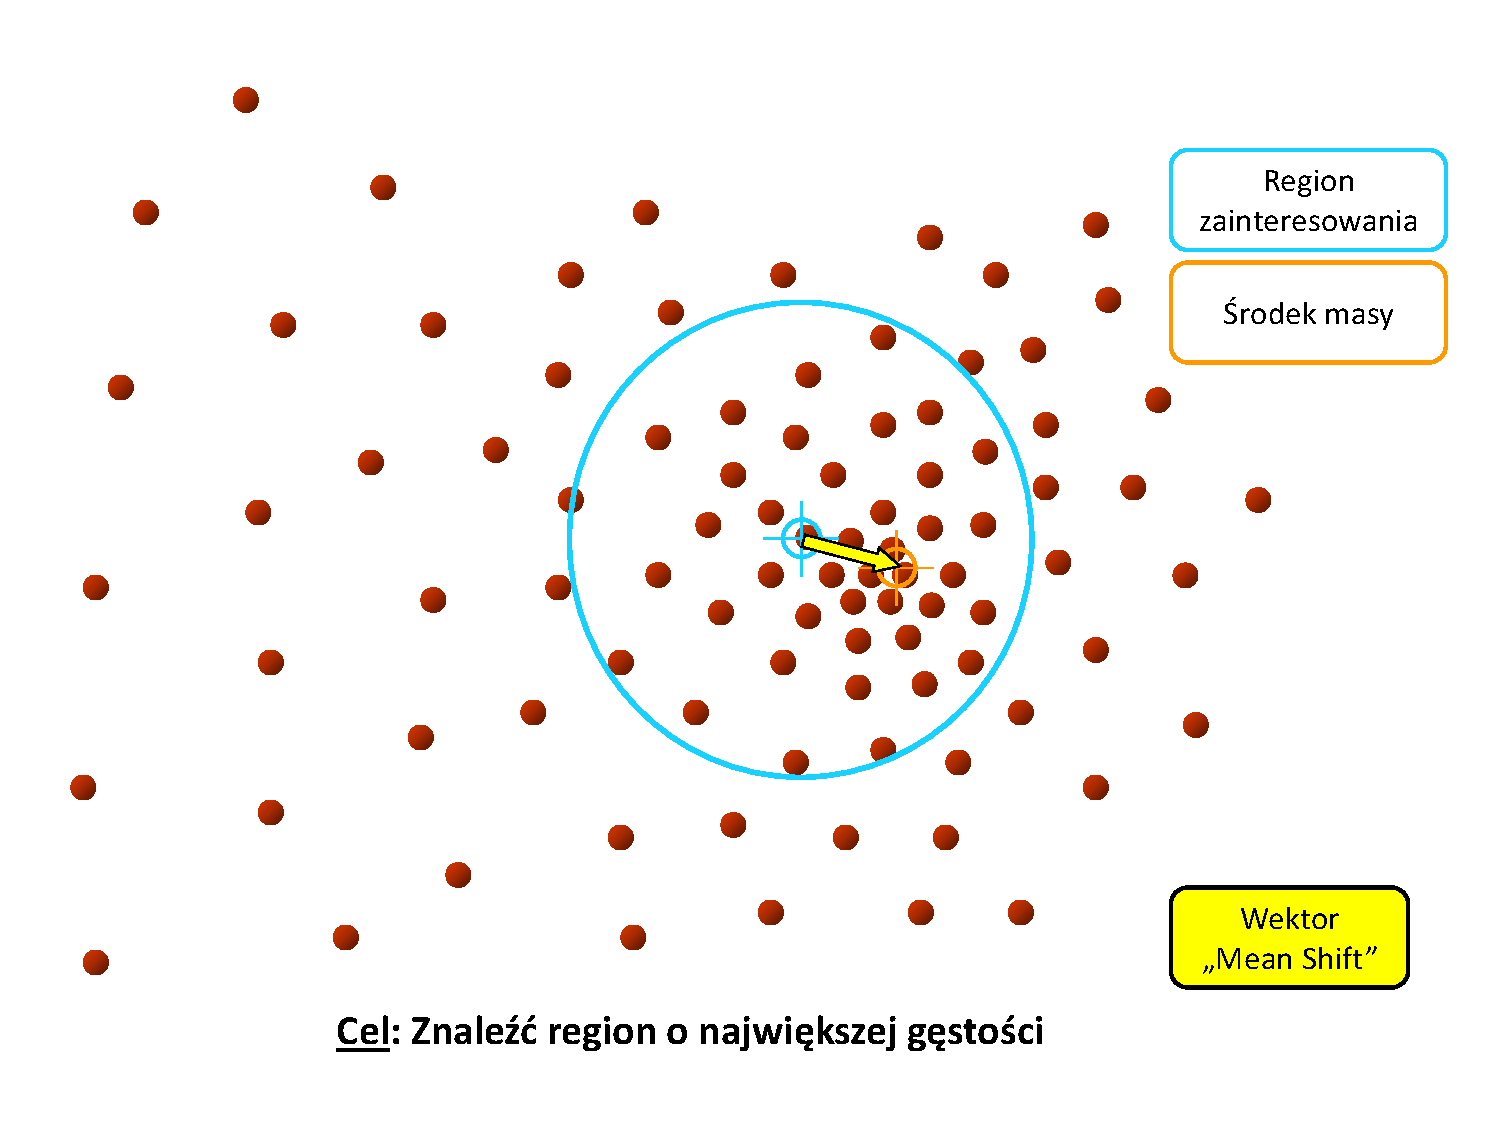
\includegraphics[width=0.9\textwidth]{mean_shift_intuitive_5.pdf}
			\adapted{\href{http://www.wisdom.weizmann.ac.il/~vision/courses/2004_2/files/mean_shift/mean_shift.ppt}{Ukrainitz, Y., Sarel, B.}}
		\end{figure}
	\end{frame}
	
	\begin{frame}
		\frametitle{Czym jest Mean Shift?}
		\framesubtitle{Podejście intuicyjne}
		\begin{figure}[H]
			\centering
			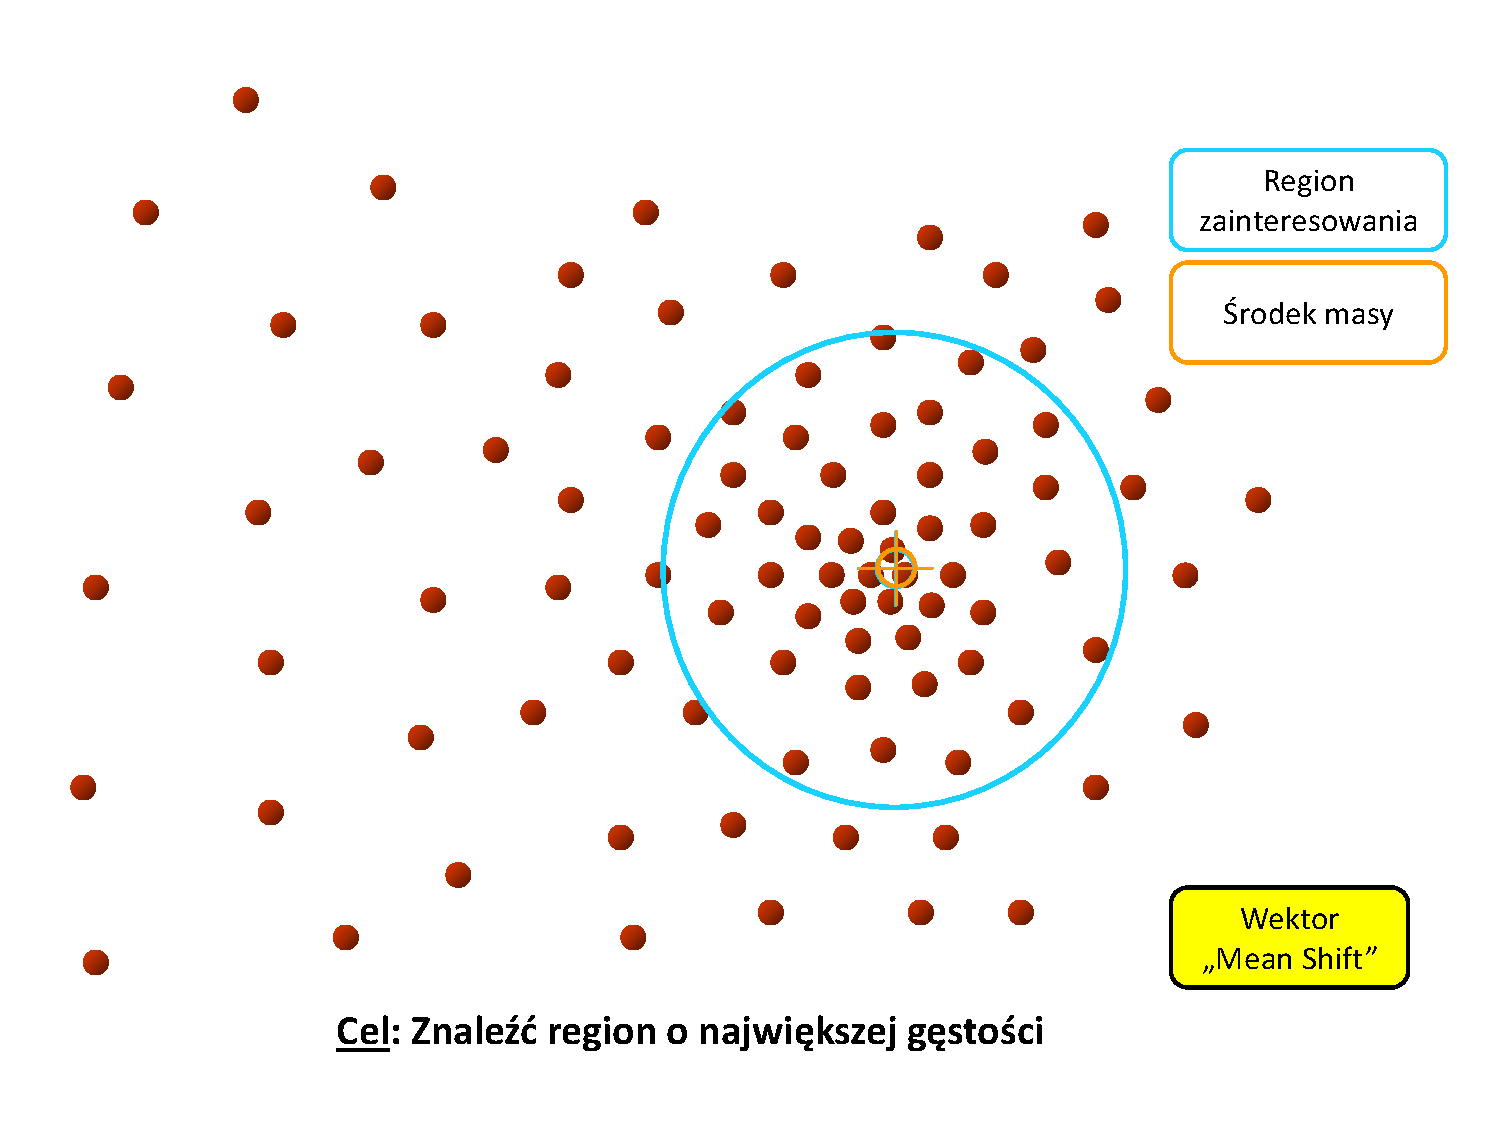
\includegraphics[width=0.9\textwidth]{mean_shift_intuitive_6.pdf}
			\adapted{\href{http://www.wisdom.weizmann.ac.il/~vision/courses/2004_2/files/mean_shift/mean_shift.ppt}{Ukrainitz, Y., Sarel, B.}}
		\end{figure}
	\end{frame}
	
	\subsection{Podejście matematyczne}
	\begin{frame}
		\begin{beamercolorbox}[colsep=-4bp,rounded=true,shadow=true,ht=1cm,dp=0.3cm,center]{title}
			\usebeamerfont{title} \usebeamercolor*[fg]{title} Czym jest Mean Shift?\\
			\usebeamerfont{subtitle} \usebeamercolor*[fg]{subtitle} Podejście matematyczne
		\end{beamercolorbox}
	\end{frame}
	
	\begin{frame}
		\frametitle{Czym jest Mean Shift?}
		\framesubtitle{Podejście matematyczne}
		Mean Shift pozwala znaleźć lokalne maksima funkcji gęstości prawdopodobieństwa (PDF - ang. \textit{Probability Density Function}) na podstawie skończonej liczby próbek.
		
		\begin{block}{Co może reprezentować PDF}
			\begin{itemize}
				\item jasność,
				\item barwę,
				\item kształt,
				\item ... praktycznie wszystko.
			\end{itemize}
		\end{block}
	\end{frame}
	
	\begin{frame}
		\frametitle{Czym jest Mean Shift?}
		\framesubtitle{KDE - ang. \textit{Kernel Density Estimation}}
		Wyznaczyć PDF na podstawie próby... ale:
		\begin{itemize}
			\item Nieznany rozkład danych \(\Rightarrow\) estymacja nieparametryczna.
		\end{itemize}
		%Należy wyznaczyć  mając do dyspozycji jedynie ograniczony zbiór wartości z populacji (próbę). Nie wiadomo z jakiego rozkładu pochodzą dane, wiec należy użyć estymatora nieparametrycznego.
		Niech \(X\) będzie \(n\)-wymiarową zmienną losową, której rozkład gęstości jest opisany przez \(f\). Jej estymator jądrowy (\textit{Kernel Density Estimator}) \(\hat{f}\) można wyznaczyć na podstawie \(m\)-elementowej próby losowej: \(x_{1},x_{2},\ldots,x_{m}\):
		\begin{equation}\label{eq:KDE}
		\hat{f}(x) = \frac{1}{m}\sum_{i=1}^{m}K\left(x - x_{i}\right)
		\end{equation}
		gdzie funkcja \(K\) jest nazywana jądrem (ang. \textit{kernel})
	\end{frame}
	
	\begin{frame}
		\frametitle{Czym jest Mean Shift?}
		\framesubtitle{Kernel function}
		\begin{equation*}\tag{\ref{eq:KDE}}
		\hat{f}(x) = \frac{1}{m}\sum_{i=1}^{m}K\left(x - x_{i}\right)
		\end{equation*}
		Funkcja \(K\) musi spełniać kilka warunków:
		\begin{itemize}
			\item jest znormalizowana:
			\[\int K(x) dx = 1\]
			\item jest symetryczna:
			\[K(-x) = K(x)\]
			\item jest nieujemna,
			\item jest ograniczona.
		\end{itemize}
	\end{frame}
	
	\begin{frame}
		\frametitle{Czym jest Mean Shift?}
		\framesubtitle{Kernel function - przykłady}
		Przykładowe funkcje jądra:
		\begin{columns}[T]
			\begin{column}{.5\textwidth}
				\begin{itemize}
					\item Epanecznikowa:
					\[K_{E}(\mathbf{x}) = \begin{cases}
												c(1 - \norm{\mathbf{x}}^{2}) & \text{dla } \norm{\mathbf{x}} \leq 1 \\
												0       & \text{dla } \mathbf{x} > 1
												\end{cases}\]
					\item Gaussa:
					\[K_{G}(\mathbf{x}) = \begin{cases}
					c \cdot \exp(-0.5\cdot\norm{\mathbf{x}}^{2}) & \text{dla } \norm{\mathbf{x}} \leq 1 \\
					0       & \text{dla } \mathbf{x} > 1
					\end{cases}\]
					\item Jednolita:
					\[K_{U}(\mathbf{x}) = \begin{cases}
					c & \text{dla } \norm{\mathbf{x}} \leq 1 \\
					0       & \text{dla } \mathbf{x} > 1
					\end{cases}\]
				\end{itemize}
			\end{column}
			\begin{column}{.5\textwidth}
				\begin{itemize}[label={}]
					\item \hspace{0.1\linewidth}
					\begin{figure}[H]
						\centering
						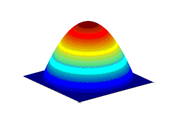
\includegraphics[width=0.35\textwidth]{epanechnikov_kernel.png}
						\source{\href{http://www.wisdom.weizmann.ac.il/~vision/courses/2004_2/files/mean_shift/mean_shift.ppt}{Ukrainitz, Y., Sarel, B.}}
					\end{figure}
					\item \hspace{0.1\linewidth}
					\begin{figure}[H]
						\centering
						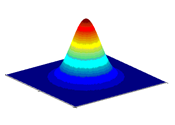
\includegraphics[width=0.35\textwidth]{normal_kernel.png}
					\end{figure}
					\item \hspace{0.1\linewidth}
					\begin{figure}[H]
						\centering
						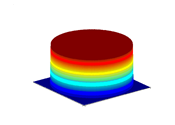
\includegraphics[width=0.35\textwidth]{uniform_kernel.png}
					\end{figure}
				\end{itemize}
			\end{column}
		\end{columns}
	\end{frame}

	\section{Algorytm}
	\begin{frame}
		\begin{beamercolorbox}[colsep=-4bp,rounded=true,shadow=true,ht=1cm,dp=0.3cm,center]{title}
			\usebeamerfont{title} \usebeamercolor*[fg]{title} Mean Shift\\
			\usebeamerfont{subtitle} \usebeamercolor*[fg]{subtitle} Algorytm
		\end{beamercolorbox}
	\end{frame}

	\begin{frame}
		\frametitle{Mean Shift}
		\framesubtitle{Algorytm}
		\begin{enumerate}
			\item Wybierz początkową pozycję i rozmiar regionu zainteresowania.
			\item Wyznacz środek gęstości cechy w regionie.
			\item Wyznacz wektor przesunięcia:
			\[
			\mathbf{m}(x) = \frac{\sum_{x_{i} \in N(x)}K(x_{i} - x) \cdot x_{i}}{\sum_{x_{i} \in N(x)}K(x_{i} - x)}
			\]gdzie \(N(x)\) to otoczenie punktu \(x\) określone przez rozmiar regionu zainteresowania.
			\item Przesuń środek regionu zainteresowania o wyznaczony wektor.
			\item Powtarzaj kroki 2. - 4. do osiągnięcia zbieżności.
		\end{enumerate}
	\end{frame}
	
	\section{Wady, zalety oraz zastosowania}
	\begin{frame}
		\begin{beamercolorbox}[colsep=-4bp,rounded=true,shadow=true,ht=1cm,dp=0.3cm,center]{title}
			\usebeamerfont{title} \usebeamercolor*[fg]{title} Mean Shift\\
			\usebeamerfont{subtitle} \usebeamercolor*[fg]{subtitle} Wady, zalety oraz zastosowania
		\end{beamercolorbox}
	\end{frame}
	
	\begin{frame}
		\frametitle{Mean Shift}
		\framesubtitle{Wady i zalety}
		\begin{columns}[T]
			\begin{column}{.5\textwidth}
				Zalety:
				\begin{itemize}
					\item Prosta implementacja,
					\item Nie zakłada określonego kształtu,
					\item Może działać w dokładnie określonej przestrzeni cech,
					\item Tylko jeden parametr musi być odgórnie podany (rozmiar okna).
				\end{itemize}
			\end{column}
			\begin{column}{.5\textwidth}
				Wady:
				\begin{itemize}
					\item Rozmiar regionu zainteresowania (okna analizy) jest ustalony z góry i nie ma żadnego sposobu na jego optymalne wyznaczenie,
					\item Źle dobrany rozmiar okna może przekreślić skuteczność algorytmu.
				\end{itemize}
			\end{column}
		\end{columns}
	\end{frame}
	
	\begin{frame}
		\frametitle{Mean Shift}
		\framesubtitle{Zastosowania}
		Zastosowania:
		\begin{itemize}
			\item Śledzenie obiektów (także w czasie rzeczywistym),
			\item Klasteryzacja (grupowanie) danych,
			\item Segmentacja obrazów,
			\item Wygładzanie zachowujące nieciągłości (krawędzie).
		\end{itemize}
	\end{frame}

	\begin{frame}
		\frametitle{Mean Shift}
		\framesubtitle{Zastosowania - segmentacja obrazu}
		\begin{figure}[H]
			\centering
			\begin{minipage}{.45\textwidth}
				\centering
				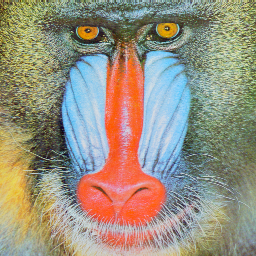
\includegraphics[width=.7\linewidth]{baboon_original.png}
				\caption{\textit{Baboon} - obraz oryginalny.}
				\source{Comaniciu, D., Meer, P.}
			\end{minipage}
			\begin{minipage}{.45\textwidth}
				\centering
				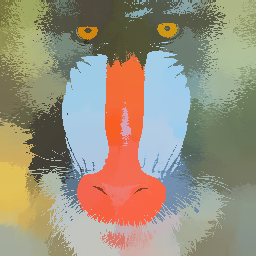
\includegraphics[width=.7\linewidth]{baboon_filtered.png}
				\caption{\textit{Baboon} - obraz poddany segmentacji.}
			\end{minipage}
			\caption{Segmentacja obrazu za pomocą Mean Shift.}
		\end{figure}
	\end{frame}
	
	\begin{frame}
		\frametitle{Mean Shift}
		\framesubtitle{Zastosowania - filtracja obrazu}
		\begin{figure}[H]
			\centering
			\begin{minipage}{.45\textwidth}
				\centering
				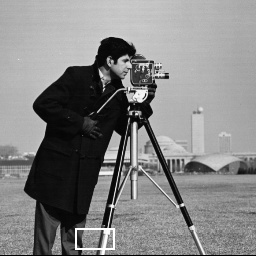
\includegraphics[width=.7\linewidth]{cameraman_original.png}
				\caption{\textit{Cameraman} - obraz oryginalny.}
				\source{Comaniciu, D., Meer, P.}
			\end{minipage}
			\begin{minipage}{.45\textwidth}
				\centering
				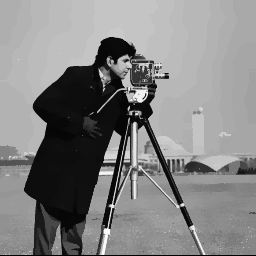
\includegraphics[width=.7\linewidth]{cameraman_filtered.png}
				\caption{\textit{Cameraman} - obraz poddany filtracji.}
			\end{minipage}
			\caption{Filtracja obrazu za pomocą Mean Shift zachowująca ostre krawędzie.}
		\end{figure}
	\end{frame}
	
	\begin{frame}
		\frametitle{Mean Shift}
		\framesubtitle{Zastosowania - klasteryzacja}
		\begin{figure}[H]
			\centering
			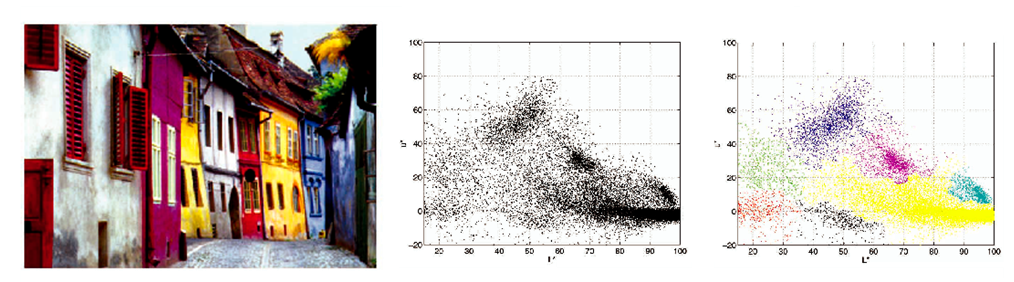
\includegraphics[width=\textwidth]{color_clustering.png}
			\caption{Klasteryzacja kolorów za pomocą algorytmu Mean Shift.}
			\source{Comaniciu, D., Meer, P.}
		\end{figure}
	\end{frame}

	\begin{frame}
		\frametitle{Mean Shift}
		\framesubtitle{Zastosowania - śledzenie obiektów}
		\begin{figure}[H]
			\centering
			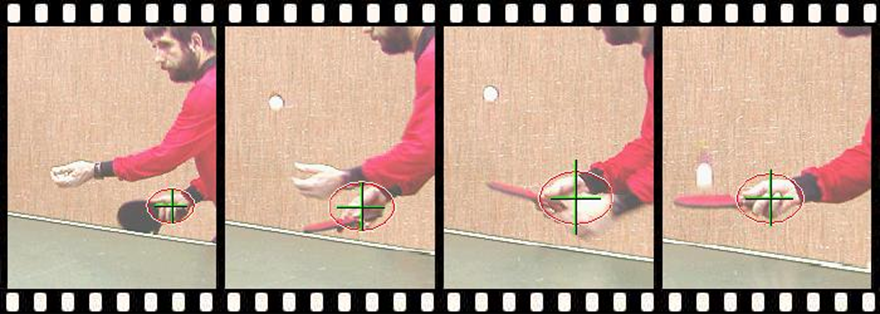
\includegraphics[width=\textwidth]{object_tracking.png}
			\caption{Śledzenie obiektów za pomocą algorytmu Mean Shift.}
			\source{\href{http://www.wisdom.weizmann.ac.il/~vision/courses/2004_2/files/mean_shift/mean_shift.ppt}{Ukrainitz, Y., Sarel, B.}}
		\end{figure}
	\end{frame}
	
	\section{Continuously Adaptive Mean Shift (CAMShift)}
	\begin{frame}
		\begin{beamercolorbox}[colsep=-4bp,rounded=true,shadow=true,ht=0.5cm,dp=0.3cm,center]{title}
			\usebeamerfont{title} \usebeamercolor*[fg]{title} Continuously Adaptive Mean Shift (CAMShift)
		\end{beamercolorbox}
	\end{frame}
	
	\begin{frame}
		\frametitle{CAMShift}
		\framesubtitle{Mean Shift - problem skali}
		\begin{itemize}
			\item Stały rozmiar okna analizy jest znaczącą wadą algorytmu Mean Shift,
			\item Rozwiązaniem jest dynamicznie zmieniający się rozmiar, czyli CAMShift.
		\end{itemize}
		
		\begin{figure}[H]
			\centering
			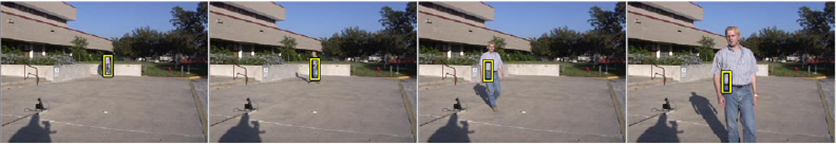
\includegraphics[width=\textwidth]{mean_shift_scale_problem.png}
			\source{\href{http://www.wisdom.weizmann.ac.il/~vision/courses/2004_2/files/mean_shift/mean_shift.ppt}{Ukrainitz, Y., Sarel, B.}}
		\end{figure}
	\end{frame}
	
	\begin{frame}
		\frametitle{CAMShift}
		\framesubtitle{Mean Shift - problem skali}
		\begin{itemize}
			\item Stały rozmiar okna analizy jest znaczącą wadą algorytmu Mean Shift,
			\item Rozwiązaniem jest dynamicznie zmieniający się rozmiar, czyli CAMShift.
		\end{itemize}
		
		\begin{figure}[H]
			\centering
			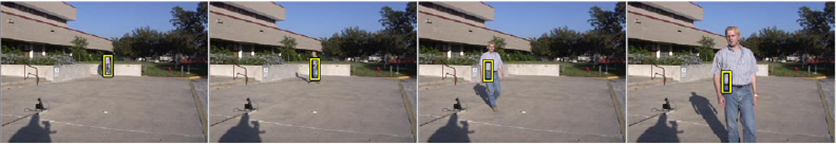
\includegraphics[width=\textwidth]{mean_shift_scale_problem.png}
			\source{\href{http://www.wisdom.weizmann.ac.il/~vision/courses/2004_2/files/mean_shift/mean_shift.ppt}{Ukrainitz, Y., Sarel, B.}}
		\end{figure}
	\end{frame}
	
	\begin{frame}
		\frametitle{CAMShift}
		\framesubtitle{CAMShift}
		Algorytm:
		\begin{enumerate}
			\item Wybierz początkową pozycję i rozmiar okna analizy.
			\item Wykonaj Mean Shift.
			\item Ustal wielkość okna w zależności od funkcji zerowego momentu rozkładu.
		\end{enumerate}
		
		\begin{figure}[H]
			\centering
			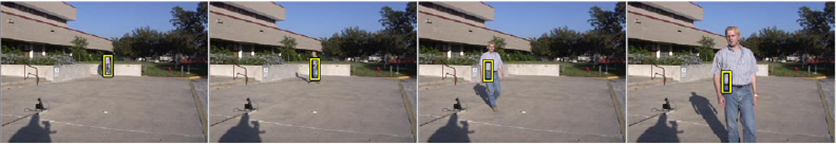
\includegraphics[width=\textwidth]{mean_shift_scale_problem.png}
			\hspace{0.1\textwidth}
			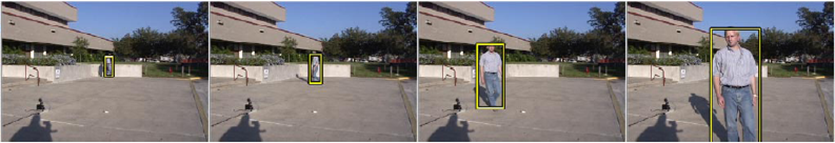
\includegraphics[width=\textwidth]{cam_shift.png}
			\source{\href{http://www.wisdom.weizmann.ac.il/~vision/courses/2004_2/files/mean_shift/mean_shift.ppt}{Ukrainitz, Y., Sarel, B.}}
		\end{figure}
	\end{frame}
	
	\section{Pytania}
	\begin{frame}
		\begin{beamercolorbox}[colsep=-4bp,rounded=true,shadow=true,ht=0.5cm,dp=0.3cm,center]{title}
			\usebeamerfont{title} \usebeamercolor*[fg]{title} Pytania
		\end{beamercolorbox}
	\end{frame}
	
	\begin{frame}
		\begin{beamercolorbox}[colsep=-4bp,rounded=true,shadow=true,ht=0.5cm,dp=0.3cm,center]{title}
			\usebeamerfont{title} \usebeamercolor*[fg]{title} Dziękuję za uwagę :)
		\end{beamercolorbox}
	\end{frame}
	
\end{document}
